% From here:
% http://laberintos.itam.mx/latex-para-tesistas-ii/

\pgfplotsset{compat=1.13}

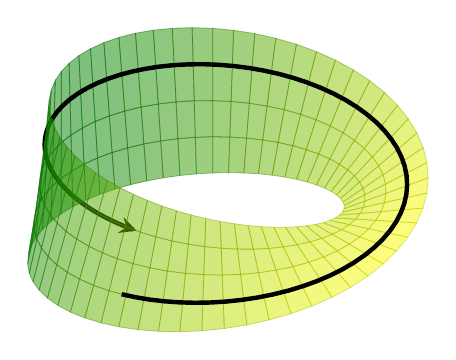
\begin{tikzpicture}

  \begin{axis}[hide axis, view={30}{50}]
  
    % backside walk, domain depends on the camera angle :-(
    \addplot3 [ultra thick, black, -stealth, samples y=0,
               samples=60, domain=188:270] (
    {(1+0.125*cos(x/2))*cos(x)},
    {(1+0.125*cos(x/2))*sin(x)},
    {0.125*sin(x/2)});

    % surface
    \addplot3 [surf, point meta=x, colormap/greenyellow, thin, line width=0.1mm, z buffer=sort, 
               samples=60, samples y=5, domain=-180:180, y domain=-0.5:0.5, opacity=0.5] 
    ({(1+0.5*y*cos(x/2))*cos(x)},
     {(1+0.5*y*cos(x/2))*sin(x)},
     {0.5*y*sin(x/2)});

    % frontside walk, domain depends on the camera angle :-(
    \addplot3 [ultra thick, black, -, samples y=0, samples=60, domain=-90:188] 
    ({(1+0.125*cos(x/2))*cos(x)},
     {(1+0.125*cos(x/2))*sin(x)},
     {0.125*sin(x/2)});
     
  \end{axis}
  
\end{tikzpicture}